\part{An Introduction to Using \LaTeX{}}

\section{What is \LaTeX{} (lay-teck) or LaTeX, but not latex or Latex?}

\begin{itemize}

\item \LaTeX{} is an open, document--preparation system used by many students,
  academics, and publishers whose content involves technical topics or complex
  structure (\textit{e.g.}\ math professors, engineers, you).

\item \LaTeX{} is a kind of markup language. This means \LaTeX{} files
  explicitly articulate both the \textit{content} and the
  \textit{structure}. Other markup languages include HTML, XML and Markdown. If
  you go to the New York Times webpage (\url{www.nytimes.com}) and view the HTML
  source for the main page it will look (incredibly) different from how that web
  page is rendered by your browser. \footnote{In the Google Chrome browser you
    can view source by navigating to the ``Tools'' menu item and choosing ``View
    Source''.} The web page is written in the HTML markup language, but then a
  separate program renders the page. The main point here is that ``creation''
  and ``consumption'' are conceptually distinct. LaTeX{} is much more similar to
  HTML source than it is to a word processor (\textit{e.g.}  MS Word, OpenOffice
  Writer, Google Documents). When you work with a \LaTeX{} file, you describe
  how the file should look, but this is not displayed for you in real-time.
\end{itemize}

\section{Why Would You Use \LaTeX{}?}

\LaTeX{} has a number of distinct advantages:

\begin{itemize}

\item A \LaTeX{} document can be very pleasing to the eye without the need for
  any customization.

\item When your focus is on producing content, but are neither a publisher nor a
  graphic designer, \LaTeX{} lets you focus on the content: \LaTeX{} separates
  content from appearance.

\item \LaTeX{}'s ability to incorporate math is un-rivaled.

% \item People in this discipline who do things like what you will do
%   will expect it.

\item You will never get locked out from the fruits of your intellectual labor
  because of licenses or old software. The software is open and the files you
  create are ``flat text'' files. If someone has a computer, they can read your
  \LaTeX{} files.

\item Also, because it relies on plain text files, collaboration among multiple
  contributors to a single project can be managed \textit{much} more readily.

\item The markup code for \LaTeX{} math is one of the canonical ways
  of representing math in plain-text environments (\textit{e.g.}\
  email, instant messaging).

\end{itemize}

\section{How Does \LaTeX{} Work?}

\par The process of creating a \LaTeX{} document is quite different from
creating one in a word processor. There is, undeniably, a learning curve.

Although most of the technical details can safely be ignored, some understanding
of the different components comprising a functioning \LaTeX{} workflow is
helpful at the outset. And, understanding how pieces fit together makes asking
for help much easier. A basic representation of the workflow is given in
Figure~\ref{fig:workflow}.

\begin{figure}
  \caption{Example \LaTeX{} Workflow}
  \label{fig:workflow}
  \begin{center}
    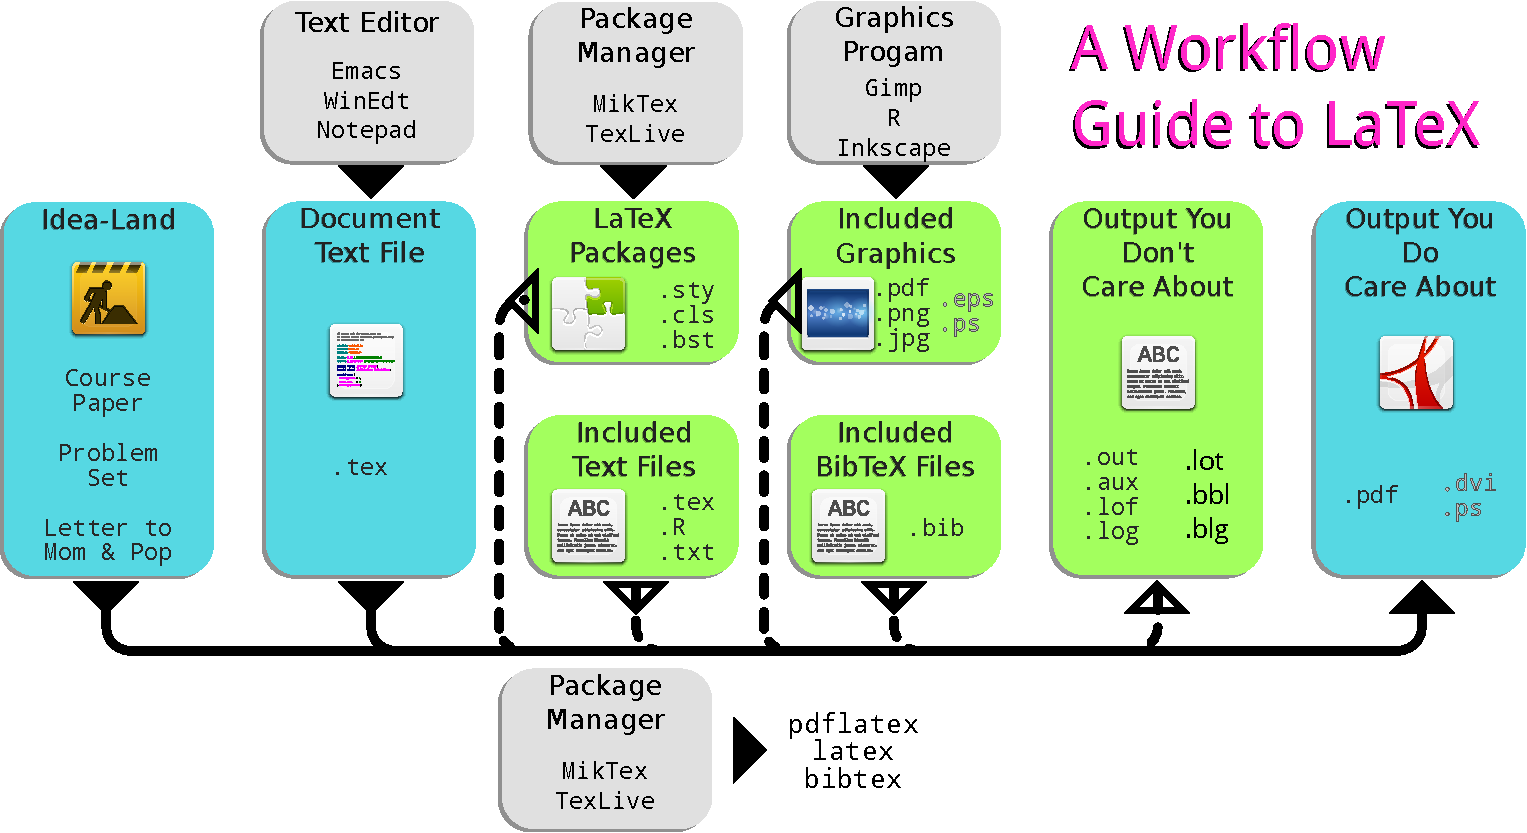
\includegraphics[scale=.5,angle=90]{./Extra_Materials/workflow.pdf}

    \blurb{An example workflow using \LaTeX{} to produce the output you care
      about. Blue regions represent the components you will focus on the most on
      a daily basis. Grey regions represent the software that will help you get
      from start to finish. Green regions represent intermediate or sometimes
      option files that are less focal.}
  \end{center}
\end{figure}


The basic steps to creating a document are:
\begin{enumerate}
\item Have an idea!

\item Create a plain text document containing the content in a text
  editor. These plain text files a typically given a file extension of
  \verb=.tex=.

\item Process the plain text document with the \LaTeX{} ``program''.

\item \LaTeX{} pulls in any additional files that are asked for---but they have
  to be asked for---and creates, among other files, the document you will print
  or email. Most of the time, this is a PDF file.

\item View the result/rendering of your \LaTeX{} document by opening the PDF
  file.

\item Be happy.

\end{enumerate}

Notice that this is different from the word processor workflow. In
that case, Steps 2, 4, and 5 are basically integrated. Step 3 is
unnecessary. Step 6 may or may not happen.

What now follows is some more explanation of the kind of software will be needed
for each step.

\paragraph{Step 2} You could use any number of other text editors. Many Windows
users like WinEdt or Sublime. Other options include nerdier text editors like
Emacs. It's best to find a text editor with well-documented \LaTeX{}
integration. This will facilitate the next steps after you write your file.

We typically denote \LaTeX{} files with the \texttt{.tex} file
extension. Although it isn't necessary in some cases, most software and
operating systems will make your life easier if you are willing to name \LaTeX{}
files what they expect you to name them.

\paragraph{Step 3} If you have chosen your text editor well, you can achieve
this from within that program. For example, WinEdt has a button you can just
click to process your \texttt{.tex} file.

\par Also, \LaTeX{}-ing your document can proceed through one of two different
branches. I will focus on the \texttt{pdflatex} branch and not the
\texttt{latex} branch. \texttt{pdflatex} will convert your \texttt{.tex} file
into a \texttt{.pdf} document. Included images must be \texttt{.jpg},
\texttt{.png}, \texttt{.pdf}, or \texttt{.svg} files. These inputs and PDF
output are far more common now, so that is the focus here.

\paragraph{Step 4} Sometimes markup in the \LaTeX{} file will require
contributed packages which tell the \LaTeX{} how the content should be
rendered. This is one of the critical benefits of using a system like \LaTeX{}:
you can utilize functionality that many other people have already provided
rather than re-invent it or do without.

However, making sure these packages are placed in the right spot on your system
and up-to-date can be involved and opaque to the newcomer. \LaTeX{} package
managers simplify this. On Window machines, MikTeX is often used. By and large,
you can and should ignore this fact in the beginning of your \LaTeX{}
experience. What is important is to realize the following:
\[
\textrm{\LaTeX{}} \neq \textrm{a text editor} \neq \textrm{a package manager
  like MikTeX}.
\]

\paragraph{Step 5} Once you have a PDF file, you can view it in your preferred
PDF viewer like Adobe Reader. A well-chosen text editor will make this viewing
easy, too.

\paragraph{Step 6} No software necessary.

\section{Exercise: Your First Document}

\begin{enumerate}
\item Go to
  \url{https://github.com/olmjo/LaTeX-Intro/tree/master/Extra_Materials}.

\item Save the file \texttt{FakeFile.tex} to your desktop.

\item Open this file in your text editor.

\item Run \texttt{pdflatex} on the \texttt{.tex} file and view it.

\item Notice how many ancillary files this process creates.

\end{enumerate}

The contents of this file are as follows:

\lstinputlisting{Extra_Materials/FakeFile.tex}

You have successfully created your first \LaTeX{} document and
simultaneously learned to always keep \LaTeX{} files/projects in
separate directories because the output will create clutter. Consider
this a windfall!


%%% Local Variables:
%%% mode: latex
%%% TeX-master: "../../tutorial"
%%% End:
